\documentclass{article}

\usepackage{graphicx} % for images
\usepackage{amsmath} % for math
\usepackage{amssymb} % for \mathbb
\usepackage{siunitx} % for \SI, \num
\usepackage{hyperref} % for \url{}

% This stuff is for figures
\usepackage{float}
\DeclareGraphicsExtensions{.pdf, .png, .jpg}

% coloring of links for PDF format
\hypersetup{
    colorlinks=true,
    urlcolor=blue,
    linkcolor=blue
}

% \c command redefinition (for monospaced font)
\renewcommand{\c}[1]{\texttt{#1}}
% \today command re-definition
% https://tex.stackexchange.com/questions/112932/today-month-as-text
\renewcommand{\today}{\ifnum\number\day<10 0\fi \number\day \space%
\ifcase \month \or January\or February\or March\or April\or May%
\or June\or July\or August\or September\or October\or November\or December\fi\space%
\number \year} 

\begin{document}

\noindent
Rodrigo Becerril Ferreyra\\
Dr. Alireza Mehrnia\\
CECS~463\\
\today

\noindent
{\centering Final Project}

\section*{Question 1}
The default filter is actually an FIR filter. This is because
its poles are all located at 0. Below is an intuitive derivation of
this fact (just one example; i.e. not a hard proof).

An FIR filter is a filter that only depends on the current and
previous inputs, and not previous outputs.

\begin{equation*}
    y[n] = b_0 x[n] + b_1 x[n-1] + b_2 x[n-2] + \cdots + b_N x[n-N]
\end{equation*}

If we take the \(z\)-transform of both sides, we can find the
transfer function and analyze the poles and zeros.

\begin{gather*}
    Y(z) = b_0 X(z) + b_1 X(z)z^{-1} + b_2X(z)z^{-2} + \cdots + b_N X(z)z^{-N}\\
    Y(z) = X(z) (b_0 + b_1 z^{-1} + b_2 z^{-2} + \cdots + b_N z^{-N})\\
    H(z) = \frac{Y(z)}{X(z)} = \frac{b_0 + b_1 z^{-1} + b_2 z^{-2} + \cdots + b_N z^{-N}}{1} \left(\frac{z^N}{z^N}\right)\\
    = \frac{b_0z^N + b_1 z^{N-1} + b_2 z^{N-2} + \cdots + b_N}{z^N}
\end{gather*}

There are \(N\) poles (and \(N\) zeros) by the Fundamental
Theorem of Algebra. In this case, all of the poles are all 0.
\(N\) is the order of the filter, so in this case,
the order is 50.

\section*{Question 2}
Several things happened when the zeros were removed:
\begin{itemize}
    \item The highest magnitude of the frequency response dropped
    from a little over 1 to 0.4. Before the deletion, there were
    50 zeros and 50 poles. With the deletion of two zeros, there
    are now less zeros than poles, which decreases the total
    magnitude of the filter.
    \item The magnitude of the frequency response near 0 normalized
    is now lower than the magnitude at the cutoff frequency
    (about 0.4 normalized). This is because, by removing poles
    close to the angle of \(\pi\), frequencies close to
    1 normalized are free to come out stronger than frequencies
    close to 0 normalized.
    \item There is now positive (as opposed to 0) magnitude at
    the maximum 1 normalized. The reason for this is the same as
    before: removing the zeros gave high frequencies more
    freedom.
    \item The argument (phase) part of the frequency response
    is left untouched. This is because we deleted both a zero
    and its conjugate.
\end{itemize}

\section*{Question 3}
The small effect of deleting the first two zeros has now been
greatly exaggerated: the filter passes signals with frequencies
close to the Nyquist rate due to the fact that there is no
zero at that frequency to suppress them. The maximum magnitude
is now a bit over 1, while the section from 0 to 0.4
normalized is now half of what it was previously.

\section*{Question 4}
This is a high-pass filter. The zero placed at \(z = 1\)
suppresses frequencies at \(\omega = 0\) because it was placed
at a point where it has 0 argument. If more zeros were placed at
this point, it would create a sharper transition between blocking
and passing frequencies.

\section*{Question 5}
Moving the zero from \(z = 1 = e^{j0}\) to \(z = e^{j\pi/4}\),
we now have complex coefficients for the filter. This is because
we are no longer adding zeros in conjugates, which makes sure to
remove the imaginary portion of the numbers. Since symmetry is
only guaranteed from \SI{0}{\hertz} to \(f_s/2\) for real
numbers, it is not applicable to this situation, and an extended
\(-f_s/2\) to \(f_s/2\) domain is used instead.

The magnitude of the frequency response now shows a dip at
\(\pi/4\) normalized, or about \SI{9.425}{\kilo\hertz}. The
maximum magnitude is 2.

\section*{Question 6}
Yes, the movement of the zero displays the expected outcome,
especially on normalized frequency mode. The dip in magnitude is
always pointed to the argument of the zero. For arguments close
to \(\pi\), There appears to be two such dips on the frequency
response, but this is simply due to the extended domain used,
and the fact that an argument of \(-\pi\) is the same as
an argument of \(\pi\).

\section*{Question 7}
The magnitude of the frequency response theoretically goes to
infinity, but this is only approximated in the filter designer
due to the finite sampling rate. It is of course very high.
This filter is no longer stable because the region of convergence
of the transfer function (\(z\)-transform) that defines this
filter does not include the circle \(|z| = 1\).
For any low frequencies (such as DC or \(\omega = 0\); i.e. a
step excitation), one can
imagine what would happen: even for a low initial value, the
output would be greatly amplified (around 2500 times for a
filter gain of 1), and the output would quickly grow in size,
constantly being added to itself due to this being an IIR filter.

Additionally,
the Filter Designer tool shows that the filter is not stable.

The spike in the magnitude definitely moves according to prediction,
just like the same experiment with the zero.

\section*{Question 8}
This filter is not stable. This can be deduced by only looking
at the frequency response; specifically, by looking at the
argument part of the frequency response. Below is the phase
response of the unstable filter. Note how the lowest value
(corresponding to frequency \(-f_s/2\) and the highest value
(corresponding to frequency \(f_s/2\)) do not match.
Due to the periodicity of the frequency response, as the graph
increases in domain (above \(f_s/2\)), the argument will
jump from about 6 to about \(-0.5\).
This means that the phase response is not continuous and
therefore not stable.

\begin{figure}[H]
    \centering
    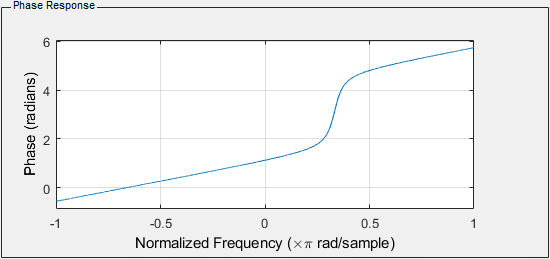
\includegraphics[width=\textwidth]{Images/unstable}
    \caption{Unstable filter. One pole at \(z = 1.1e^{j\pi/3}\).}
    \label{plot:unstable phase}
\end{figure}

\section*{Question 9}
This filter is indeed stable. This can be deduced by looking at
the phase response of the filter, as seen below. In this
example, the phase starts at \(-0.5\) at frequency \(-f_s/2\)
and ends at \(-0.5\) at frequency \(f_s/2\). In addition,
the two derivatives at the point (quantitatively) appear the
same. This leads to a nice transition as the frequency
response transitions to a new period.

\begin{figure}[H]
    \centering
    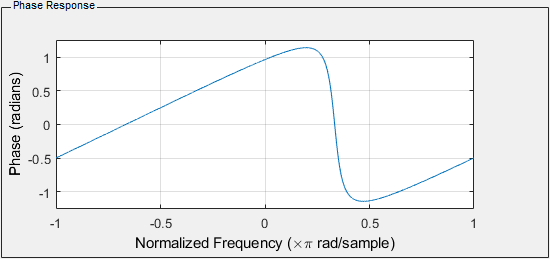
\includegraphics[width=\textwidth]{Images/stable}
    \caption{Stable filter. One pole at \(z=\frac{1}{1.1}e^{j\pi/3}\).}
    \label{plot:stable phase}
\end{figure}

\section*{Question 10}
To find the coefficients of the transfer function, I will use
the \c{poly} function available in MATLAB. The zeros are the
roots of the numerator polynomial, and the poles are the roots
of the denominator polynomial. Our zeros are
\(\{0 + 0j, 0 + 0j\}\), and our poles are
\(\{\left(1-10^{-2.275}\right) e^{\pm j5\pi /8}\}\).
In addition, my gain is 1.
Thus, the transfer function comes out to be equation
\eqref{transfer function}.

\begin{equation}\label{transfer function}
    H(z) = \frac{1z^2 + 0z + 0}{1z^2 + 0.7613z + 0.9894} = \frac{1}{1 + 0.7613z^{-1} + 0.9894z^{-2}}
\end{equation}

\begin{figure}[H]
    \centering
    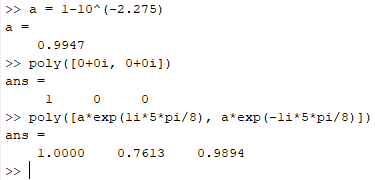
\includegraphics{Images/polynomials}
    \caption{Finding the coefficients of both polynomials.}
    \label{code:poly}
\end{figure}

\section*{Question 11}
From the filter designer export, the actual coefficients
of the filter are \(\left[ 1, 0, 0 \right]\) for the numerator
and \(\left[1,0.761303651104029,0.989410494944693\right]\) for
the denominator, so my expected values are correct.

\end{document}
